%
% This document contains the chapter about transient analysis.
%
% Copyright (C) 2003, 2004, 2006 Stefan Jahn <stefan@lkcc.org>
%
% Permission is granted to copy, distribute and/or modify this document
% under the terms of the GNU Free Documentation License, Version 1.1
% or any later version published by the Free Software Foundation.
%

\chapter{Transient Analysis}
%\addcontentsline{toc}{chapter}{Transient Analysis}

The transient simulation is the calculation of a networks response on
arbitrary excitations.  The results are network quantities (branch
currents and node voltages) as a function of time.  Substantial for
the transient analysis is the consideration of energy storing
components, i.e. inductors and capacitors.

\addvspace{12pt}

The relations between current and voltage of ideal capacitors and
inductors are given by
\begin{equation}
V_C(t) = \dfrac{1}{C}\int I_C(t) \cdot dt
\;\;\;\; \textrm{ and } \;\;\;\;
I_L(t) = \dfrac{1}{L}\int V_L(t) \cdot dt
\end{equation}

or in terms of differential equations
\begin{equation}
I_C(t) = C\cdot \dfrac{d V_C}{d t}
\;\;\;\; \textrm{ and } \;\;\;\;
V_L(t) = L\cdot \dfrac{d I_L}{d t}
\end{equation}

To calculate these quantities in a computer program numerical
integration methods are required.  With the current-voltage relations
of these components at hand it is possible to apply the modified nodal
analysis algorithm in order to calculate the networks response.  This
means the transient analysis attempts to find an approximation to the
analytical solution at discrete time points using numeric integration.

\section{Integration methods}
%\addcontentsline{toc}{section}{Integration methods}
\label{sec:IntegrationMethods}

The following differential equation is going to be solved.
\begin{equation}
\dfrac{d x}{d t} = \dot{x}(t) = f(x,t)
\label{eq:IntEquation}
\end{equation}

This differential equation is transformed into an algorithm-dependent
finite difference equation by quantizing and replacing
\begin{equation}
\dot{x}(t) = \lim_{h \rightarrow 0} \dfrac{x(t+h) - x(t)}{h}
\end{equation}

by the following equation.
\begin{equation}
\dot{x}^n = \dfrac{x^{n+1} - x^{n}}{h^{n}}
\end{equation}

There are several linear single- and multi-step numerical integration
methods available, each having advantages and disadvantages concerning
aspects of stability and accuracy.  Integration methods can also be
classified into implicit and explicit methods.  Explicit methods are
inexpensive per step but limited in stability and therefore not used
in the field of circuit simulation to obtain a correct and stable
solution.  Implicit methods are more expensive per step, have better
stability and therefore suitable for circuit simulation.

\subsection{Properties of numerical integration methods}
%\addcontentsline{toc}{subsection}{Properties of numerical integration methods}

Beforehand some definitions and explanations regarding the terms often
used in the following sections are made in order to avoid bigger
confusions later on.

\begin{itemize}
\item step size\\
The step size is defined by the arguments difference of successive
solution vectors, i.e. the time step $h^n$ during transient analysis
with $n$ being the $n$-th integration step.
\begin{equation}
h^n = t^{n+1} - t ^n
\end{equation}

\item order\\
The order $k$ of an integration method is defined as follows: With two
successive solution vectors $x^{n+1}$ and $x^{n}$ given, the successor
$x^{n+1}$ can be expressed by $x^{n}$ by a finite Taylor series.  The
order of an integrations method equals the power of the step size up
to which the approximate solution of the Taylor series differs less
than $x^{n}$ from the true solution $x^{n+1}$.

\item truncation error\\
The truncation error $\varepsilon_T$ depends on the order $k$ of the
integration method and results from the remainder term of the Taylor
series.

\item stability\\
In order to obtain an accurate network solution integration methods
are required to be stable for a given step size $h$.  Various
stability definitions exist.  This property is explained more in
detail in the following sections.  Basically it determines the
usability of an integration algorithm.

\item single- and multistep methods\\
Single step methods only use $x^n$ in order to calculate $x^{n+1}$,
multi step methods use $x^i$ with $0 \le i < n$.

\item implicit and explicit methods\\
When using explicit integration methods the evaluation of the
integration formula is sufficient for each integration step.  With
implicit methods at hand it is necessary to solve an equation system
(with non-linear networks a non-linear equation system) because for
the calculation of $x^{n+1}$, apart from $x^n$ and $\dot{x}^n$, also
$\dot{x}^{n+1}$ is used.  For the transient analysis of electrical
networks the implicit methods are better qualified than the explicit
methods.
\end{itemize}

\subsection{Elementary Methods}
%\addcontentsline{toc}{subsection}{Elementary Methods}

\subsubsection{Backward Euler}
%\addcontentsline{toc}{subsubsection}{Backward Euler}

In the implicit Euler method the right hand side of
eq. \eqref{eq:IntEquation} is substituted by $f(x^{n+1}, t^{n+1})$
which yields
\begin{equation}
\label{eq:BEInt}
f(x,t) = f(x^{n+1}, t^{n+1})
\;\;\;\; \rightarrow \;\;\;\;
x^{n+1} = x^n + h^n\cdot f(x^{n+1}, t^{n+1})
\end{equation}

The backward euler integration method is a first order single-step
method.

\subsubsection{Forward Euler}
%\addcontentsline{toc}{subsubsection}{Forward Euler}

In the explicit Euler method the right hand side of
eq. \eqref{eq:IntEquation} is substituted by $f(x^{n}, t^{n})$ which
yields
\begin{equation}
f(x,t) = f(x^n, t^n)
\;\;\;\; \rightarrow \;\;\;\;
x^{n+1} = x^n + h^n\cdot f(x^n, t^n)
\end{equation}

The explicit Euler method has stability problems.  The step size is
limited by stability.  In general explicit time marching integration
methods are not suitable for circuit analysis where computation with
large steps may be necessary when the solution changes slowly
(i.e. when the accuracy does not require small steps).

\subsubsection{Trapezoidal method}
%\addcontentsline{toc}{subsubsection}{Trapezoidal method}

For the bilinear (also called trapezoidal) integration method $f(x,t)$
is substituted by
\begin{equation}
f(x,t) = \dfrac{1}{2}\cdot \left(f(x^{n+1}, t^{n+1}) + f(x^{n}, t^{n})\right)
\end{equation}

which yields
\begin{equation}
\label{eq:TRInt}
x^{n+1} = x^n + \dfrac{h^n}{2}\cdot \left(f(x^{n+1}, t^{n+1}) + f(x^{n}, t^{n})\right)
\end{equation}

In each integration step the average value of the intervals beginning
and end is taken into account.  The trapezoidal rule integration
method is a second order single-step method.  There is no more
accurate second order integration method than the trapezoidal method.

\begin{center}
\begin{figure}[ht]
\begin{minipage}[t]{0.33\linewidth}
\centering
\includegraphics[height=1.8cm]{feuler}
forward-euler
\end{minipage}
\begin{minipage}[t]{0.33\linewidth}
\centering
\includegraphics[height=1.8cm]{beuler}
backward-euler
\end{minipage}
\begin{minipage}[t]{0.33\linewidth}
\centering
\includegraphics[height=1.8cm]{trapez}
trapezoidal
\end{minipage}
\end{figure}
\FloatBarrier
\end{center}

\subsection{Linear Multistep Methods}
%\addcontentsline{toc}{subsection}{Linear Multistep Methods}

For higher order multi-step integration methods the general purpose
method of resolution for the equation $\dot{x} = f(x,t)$
\begin{equation}
\label{eq:GenPurposeInt}
x^{n+1} = \sum^p_{i=0} a_i\cdot x^{n-i} + h \sum^p_{i=-1} b_i\cdot f(x^{n-i}, t^{n-i})
\end{equation}

is used.  With $b_{-1} = 0$ the method is explicit and therefore not
suitable for obtaining the correct and stable solution.  When $b_{-1}
\ne 0$ the method is implicit and suitable for circuit simulation,
i.e. suitable for solving stiff problems.  For differential equation
systems describing electrical networks the eigenvalues strongly vary.
These kind of differential equation systems are called stiff.

\addvspace{12pt}

For a polynom of order $k$ the number of required coefficients is
\begin{equation}
\label{eq:MultiStepCondition}
2p + 3 \ge k + 1
\end{equation}

The $2p +3$ coeffcients are choosen to satisfy
\begin{equation}
x^{n+1} = x(t^{n+1})
\end{equation}

This can be achieved by the following equation system
\begin{equation}
\begin{split}
\label{eq:MultiStepSys}
\sum^p_{i=0} a_i = 1\\
\sum^p_{i=1} (-i)^j a_i + j \sum^p_{i=-1} (-i)^{j-1} b_i = 1 & \textrm{ for } j = 1\ldots k
\end{split}
\end{equation}

The different linear multistep integration methods which can be
constructed by the equation system \eqref{eq:MultiStepSys} vary in the
equality condition corresponding with \eqref{eq:MultiStepCondition}
and the choice of coefficients which are set to zero.

\subsubsection{Gear}
%\addcontentsline{toc}{subsubsection}{Gear}

The Gear \cite{Gear} formulae (also called BDF - backward
differentiation formulae) have great importance within the multi-step
integration methods used in transient analysis programs.  The
conditions
\begin{equation}
p = k - 1
\;\;\;\; \textrm{ and } \;\;\;\;
b_0 = b_1 = \ldots = b_{k-1} = 0
\end{equation}

due to the following equation system
\begin{equation}
\label{eq:GearCoeff}
\left[\begin{array}{lrrrr}
0 & 1 &  1 &  1 &   1\\
1 & 0 & -1 & -2 &  -3\\
2 & 0 &  1 &  4 &   9\\
3 & 0 & -1 & -8 & -27\\
4 & 0 &  1 & 16 &  81\\
\end{array}\right]
\cdot
\begin{bmatrix}
b_{-1}\\
a_0\\
a_1\\
a_2\\
a_3\\
\end{bmatrix}
=
\begin{bmatrix}
1\\
1\\
1\\
1\\
1\\
\end{bmatrix}
\end{equation}

for the Gear formulae of order $4$.  Order $k = 1$ yields the implicit
Euler method.  The example given in the equation system
\eqref{eq:GearCoeff} results in the following integration formula.
\begin{equation}
\label{eq:GearInt}
\begin{split}
x^{n+1} &= a_0\cdot x^{n} + a_1\cdot x^{n-1} + a_2\cdot x^{n-2} + a_3\cdot x^{n-3} + h\cdot b_{-1}\cdot f(x^{n+1}, t^{n+1})\\
&= \dfrac{48}{25}\cdot x^{n} - \dfrac{36}{25}\cdot x^{n-1} + \dfrac{16}{25}\cdot x^{n-2} - \dfrac{3}{25}\cdot x^{n-3} + h\cdot \dfrac{12}{25}\cdot f(x^{n+1}, t^{n+1})
\end{split}
\end{equation}

There is no more stable second order integration method than the
Gear's method of second order.  Only implicit Gear methods with order
$k \le 6$ are zero stable.

\subsubsection{Adams-Bashford}
%\addcontentsline{toc}{subsubsection}{Adams-Bashford}

The Adams-Bashford algorithm is an explicit multi-step integration
method whence
\begin{equation}
p = k - 1
\;\;\;\; \textrm{ and } \;\;\;\;
a_1 = a_2 = \ldots = a_{k-1} = 0
\;\;\;\; \textrm{ and } \;\;\;\;
b_{-1} = 0
\end{equation}

is set to satisfy the equation system \eqref{eq:MultiStepSys}.  The
equation system of the Adams-Bashford coefficients of order 4 is as
follows.
\begin{equation}
\left[\begin{array}{lrrrr}
1 & 0 &  0 &   0 &    0\\
0 & 1 &  1 &   1 &    1\\
0 & 0 & -2 &  -4 &   -6\\
0 & 0 &  3 &  12 &   27\\
0 & 0 & -4 & -32 & -108\\
\end{array}\right]
\cdot
\begin{bmatrix}
a_0\\
b_0\\
b_1\\
b_2\\
b_3\\
\end{bmatrix}
=
\begin{bmatrix}
1\\
1\\
1\\
1\\
1\\
\end{bmatrix}
\end{equation}

This equation system results in the following integration formula.
\begin{equation}
\begin{split}
x^{n+1} &= a_0\cdot x^{n} + h\cdot b_{0}\cdot f^{n} + h\cdot b_{1}\cdot f^{n-1} + h\cdot b_{2}\cdot f^{n-2} + h\cdot b_{3}\cdot f^{n-3}\\
&= x^{n} + h\cdot \dfrac{55}{24}\cdot f^{n} - h\cdot \dfrac{59}{24}\cdot f^{n-1} + h\cdot \dfrac{37}{24}\cdot f^{n-2} - h\cdot \dfrac{9}{24}\cdot f^{n-3}\\
\end{split}
\end{equation}

The Adams-Bashford formula of order 1 yields the (explicit) forward
Euler integration method.

\subsubsection{Adams-Moulton}
%\addcontentsline{toc}{subsubsection}{Adams-Moulton}

The Adams-Moulton algorithm is an implicit multi-step integration
method whence
\begin{equation}
p = k - 2
\;\;\;\; \textrm{ and } \;\;\;\;
a_1 = a_2 = \ldots = a_{k-2} = 0
\end{equation}

is set to satisfy the equation system \eqref{eq:MultiStepSys}.  The
equation system of the Adams-Moulton coefficients of order 4 is as
follows.
\begin{equation}
\left[\begin{array}{lrrrr}
1 & 0 &  0 &   0 &    0\\
0 & 1 &  1 &   1 &    1\\
0 & 2 &  0 &  -2 &   -4\\
0 & 3 &  0 &   3 &   12\\
0 & 4 &  0 &  -4 &  -32\\
\end{array}\right]
\cdot
\begin{bmatrix}
a_0\\
b_{-1}\\
b_0\\
b_1\\
b_2\\
\end{bmatrix}
=
\begin{bmatrix}
1\\
1\\
1\\
1\\
1\\
\end{bmatrix}
\end{equation}

This equation system results in the following integration formula.
\begin{equation}
\label{eq:MoultonInt}
\begin{split}
x^{n+1} &= a_0\cdot x^{n} + h\cdot b_{-1}\cdot f^{n+1} + h\cdot b_{0}\cdot f^{n} + h\cdot b_{1}\cdot f^{n-1} + h\cdot b_{2}\cdot f^{n-2}\\
&= x^{n} + h\cdot \dfrac{9}{24}\cdot f^{n+1} + h\cdot \dfrac{19}{24}\cdot f^{n} - h\cdot \dfrac{5}{24}\cdot f^{n-1} + h\cdot \dfrac{1}{24}\cdot f^{n-2}\\
\end{split}
\end{equation}

The Adams-Moulton formula of order 1 yields the (implicit) backward
Euler integration method and the formula of order 2 yields the
trapezoidal rule.

\subsection{Stability considerations}
%\addcontentsline{toc}{subsection}{Stability considerations}

When evaluating the numerical formulations given for both implicit and
explicit integration formulas once rounding errors are unavoidable.
For small values of $h$ the evaluation must be repeated very often and
thus the rounding error possibly accumulates.  With higher order
algorithms it is possible to enlarge the step width and thereby reduce
the error accumulation.

\addvspace{12pt}

On the other hand it is questionable whether the construction of
implicit algorithms is really valuable because of the higher
computation effort caused by the necessary iteration (indices
$~^{n+1}$ on both sides of the equation).  In practice there is a class
of differential equations which can be reasonably handled by implicit
algorithms where explicit algorithms completely fail because of the
impracticable reduction of the step width.  This class of differential
equations are called stiff problems.  The effect of stiffness causes
for small variations in the actual solution to be computed very large
deviations in the solution which get damped.

\addvspace{12pt}

The numerical methods used for the transient analysis are required to
be stiffly stable and accurate as well.  The regions requirements in
the complex plane are visualized in the following figure.

\begin{figure}[ht]
\begin{center}
\psfrag{Re(lh)}{$\mathrm{Re \left\{h\lambda\right\}}$}
\psfrag{Im(lh)}{$\mathrm{Im \left\{h\lambda\right\}}$}
\includegraphics[width=0.7\linewidth]{stiffstable}
\end{center}
\caption{stability requirements for stiff differential equation systems}
\label{fig:StiffStable}
\end{figure}
\FloatBarrier

For values of $h\lambda$ in region II the numerical method must be
stable and accurate, in region I accurate and in region III only
stable.  The area outside the specified regions are of no particular
interest.

\addvspace{12pt}

For the stability prediction of integration algorithms with regard to
nonlinear differential equations and equation systems the simple and
linear test differential equation
\begin{equation}
\dot{x} = \lambda x
\;\;\;\; \textrm{ with } \;\;\;\;
\lambda \in \mathbb{C}, \text{Re}\left\{\lambda\right\} < 0, x \ge 0
\end{equation}

is used.  The condition $\text{Re}\left\{\lambda\right\} < 0$ ensures
the solution to be decreasing.  The general purpose method of
resolution given in \eqref{eq:GenPurposeInt} can be solved by the
polynomial method setting
\begin{equation}
x^k = z^k
\;\;\;\; \textrm{ with } \;\;\;\;
z \in \mathbb{C}
\end{equation}

Thus we get the characteristic polynom
\begin{align}
\label{eq:characteristicPolynom}
\varphi\left(z\right) &= \varrho\left(z\right) + h\lambda \cdot \eta\left(z\right) = 0\\
&= \sum^{n-1}_{i=-1} a_i\cdot z^{n-i} + h\lambda \sum^{n-1}_{i=-1} b_i\cdot z^{n-i}
\end{align}

Because of the conditions defined by \eqref{eq:MultiStepSys} the above
eq. \eqref{eq:characteristicPolynom} can only be true for
\begin{equation}
\left|z\right| < 1
\end{equation}

which describes the inner unity circle on the complex plane.  In order
to compute the boundary of the area of absolute stability it is
necessary to calculate
\begin{equation}
\label{eq:StabArea}
\mu\left(z\right) = h\lambda = -\dfrac{\varrho\left(z\right)}{\eta\left(z\right)}
\;\;\;\; \textrm{ with } \;\;\;\;
z = e^{j\vartheta}, 0 \le \vartheta \le 2\pi
\end{equation}

These equations describe closed loops. The inner of these loops
describe the area of absolute stability.  Because $\lambda \le 0$ and
$h \ge 0$ only the left half of the complex plane is of particular
interest.  An integration algorithm is call zero-stable if the
stability area encloses $\mu = 0$.  Given this condition the algorithm
is as a matter of principle usable, otherwise not.  If an algorithms
stability area encloses the whole left half plane it is called
A-stable.  A-stable algorithms are stable for any $h$ and all $\lambda
< 0$.  Any other kind of stability area introduces certain
restrictions for $\mu$.

\begin{figure}[ht]
\begin{center}
\psfrag{Re(lh)}{$\mathrm{Re \left\{h\lambda\right\}}$}
\psfrag{Im(lh)}{$\mathrm{Im \left\{h\lambda\right\}}$}
\includegraphics[width=1\linewidth]{stabgear}
\end{center}
\caption{areas of absolute stability for order 1\ldots 6 Gear formulae}
\label{fig:StabGear}
\end{figure}
\FloatBarrier

\begin{figure}[ht]
\begin{center}
\psfrag{Re(lh)}{$\mathrm{Re \left\{h\lambda\right\}}$}
\psfrag{Im(lh)}{$\mathrm{Im \left\{h\lambda\right\}}$}
\includegraphics[width=1\linewidth]{stabmoulton}
\end{center}
\caption{areas of absolute stability for order 1\ldots 6 Adams-Moulton formulae}
\label{fig:StabMoulton}
\end{figure}
\FloatBarrier

\begin{figure}[ht]
\begin{center}
\psfrag{Re(lh)}{$\mathrm{Re \left\{h\lambda\right\}}$}
\psfrag{Im(lh)}{$\mathrm{Im \left\{h\lambda\right\}}$}
\includegraphics[width=1\linewidth]{stabbashford}
\end{center}
\caption{areas of absolute stability for order 1\ldots 6 Adams-Bashford formulae}
\label{fig:StabBashford}
\end{figure}
\FloatBarrier

The figures \ref{fig:StabGear}, \ref{fig:StabMoulton} and
\ref{fig:StabBashford} visualize the evaluation of
eq. \eqref{eq:StabArea} for the discussed integration methods.  All of
the implicit formulae are zero-stable, thus principally usable.  The
(implicit) backward Euler, Gear order 2 and the trapezoidal
integration methods are A-stable.  Fig. \ref{fig:StabGear} shows why
the Gear formulae are of such great importance for the transient
analysis of electrical networks.  With least restrictions for $\mu$
they can be stabilized.

\section{Predictor-corrector methods}
%\addcontentsline{toc}{section}{Predictor-corrector methods}

In section \ref{sec:IntegrationMethods} on pages
\pageref{sec:IntegrationMethods} ff. various integration methods have
been discussed.  The elementary as well as linear multistep methods
(in order to get more accurate methods) always assumed $a_{-1} = -1$
in its general form.  Explicit methods were encountered by $b_{-1} =
0$ and implicit methods by $b_{-1} \ne 0$.  Implicit methods have been
shown to have a limited area of stability and explicit methods to have
a larger range of stability.  With increasing order $k$ the linear
multistep methods interval of absolute stability (intersection of the
area of absolute stability in the complex plane with the real axis)
decreases except for the implicit Gear formulae.

\addvspace{12pt}

For these given reasons implicit methods can be used to obtain
solutions of ordinary differential equation systems describing so
called stiff problems.  Now considering e.g. the implicit
Adams-Moulton formulae of order 3
\begin{equation}
\label{eq:AM3}
x^{n+1} = x^{n} + h\cdot \dfrac{5}{12}\cdot f^{n+1} + h\cdot \dfrac{8}{12}\cdot f^{n} - h\cdot \dfrac{1}{12}\cdot f^{n-1}
\end{equation}

clarifies that $f^{n+1}$ is necessary to calculate $x^{n+1}$ (and the
other way around as well).  Every implicit integration method has this
particular property.  The above equation can be solved using
iteration.  This iteration is said to be convergent if the integration
method is consistent and zero-stable.  A linear multistep method that
is at least first-order is called a consistent method.  Zero-stability
and consistency are necessary for convergence.  The converse is also
true.

\addvspace{12pt}

The iteration introduces a second index $m$.
\begin{equation}
\label{eq:AM3iterate}
x^{n+1,m+1} = x^{n} + h\cdot \dfrac{5}{12}\cdot f^{n+1,m} + h\cdot \dfrac{8}{12}\cdot f^{n} - h\cdot \dfrac{1}{12}\cdot f^{n-1}
\end{equation}

This iteration will converge for an arbitrary initial guess
$x^{n+1,0}$ only limited by the step size $h$.  In practice successive
iterations are processed unless
\begin{equation}
\left|x^{n+1,m+1} - x^{n+1,m}\right| < \varepsilon_{abs} + \varepsilon_{rel}\cdot \left|x^{n+1,m}\right|
\end{equation}

The disadvantage for this method is that the number of iterations
until it converges is unknown.  Alternatively it is possible to use a
fixed number of correction steps.  A cheap way of providing a good
initial guess $x^{n+1,0}$ is using an explicit integration method,
e.g. the Adams-Bashford formula of order 3.
\begin{equation}
\label{eq:AB3}
x^{n+1,0} = x^{n} + h\cdot \dfrac{23}{12}\cdot f^{n} - h\cdot \dfrac{16}{12}\cdot f^{n-1} + h\cdot \dfrac{5}{12}\cdot f^{n-2}
\end{equation}

Equation \eqref{eq:AB3} requires no iteration process and can be used
to obtain the initial guess.  The combination of evaluating a single
explicit integration method (the predictor step) in order to provide a
good initial guess for the successive evaluation of an implicit method
(the corrector step) using iteration is called predictor-corrector
method.  The motivation using an implicit integration method is its
fitness for solving stiff problems.  The explicit method (though
possibly unstable) is used to provide a good initial guess for the
corrector steps.

\subsection{Order and local truncation error}
%\addcontentsline{toc}{subsection}{Order and local truncation error}

The order of an integration method results from the truncation error
$\varepsilon_T$ which is defined as
\begin{equation}
\varepsilon_T = x\left(t^{n+1}\right) - x^{n+1}
\end{equation}

meaning the deviation of the exact solution $x\left(t^{n+1}\right)$
from the approximate solution $x^{n+1}$ obtained by the integration
method.  For explicit integration methods with $b_{-1} = 0$ the local
truncation error $\varepsilon_{LTE}$ yields
\begin{equation}
\varepsilon_{LTE} = x\left(t^{n+1}\right) - x^{n+1}
\end{equation}

and for implicit integration methods with $b_{-1} \ne 0$ it is
\begin{equation}
\varepsilon_{LTE} \approx x\left(t^{n+1}\right) - x^{n+1}
\end{equation}

Going into equation \eqref{eq:GenPurposeInt} and setting $a_{-1} = -1$
the truncation error is defined as
\begin{equation}
\label{eq:LTE}
\varepsilon_{LTE} = \sum^p_{i=-1} a_i\cdot x\left(t^{n-i}\right) + h \sum^p_{i=-1} b_i\cdot f(x\left(t^{n-i}\right), t^{n-i})
\end{equation}

With the Taylor series expansions
\begin{align}
x\left(t^{n+i}\right) &= x\left(t^{n}\right) + \dfrac{\left(ih\right)}{1!} \dot{x}\left(t^{n}\right) + \dfrac{\left(ih\right)^2}{2!} \ddot{x}\left(t^{n}\right) + \ldots\\
f(x\left(t^{n+i}\right), t^{n+i}) = \dot{x}\left(t^{n+i}\right) &= \dot{x}\left(t^{n}\right) + \dfrac{\left(ih\right)}{1!} \ddot{x}\left(t^{n}\right) + \dfrac{\left(ih\right)^2}{2!} \dddot{x}\left(t^{n}\right) + \ldots
\end{align}

the local truncation error as defined by eq. \eqref{eq:LTE} can be
written as
\begin{equation}
\varepsilon_{LTE} = C_0\cdot x\left(t^n\right) + C_1 h\cdot \dot{x}\left(t^n\right) + C_2 h^2\cdot \ddot{x}\left(t^n\right) + \ldots
\end{equation}

The error terms $C_0$, $C_1$ and $C_2$ in their general form can then
be expressed by the following equation.
\begin{equation}
\label{eq:ErrorConstant}
C_{q} = -\dfrac{1}{q!}\cdot \sum_{i=-1}^{p-1} a_i\cdot \left(p - i\right)^{q} - \dfrac{1}{\left(q - 1\right)!} \sum_{i=-1}^{p-1} b_i\cdot \left(p - i\right)^{q - 1}
\end{equation}

A linear multistep integration method is of order $k$ if
\begin{equation}
\varepsilon_{LTE} = C_{k+1}\cdot h^{k+1}\cdot x^{(k+1)}\left(t^n\right) + O\left(h^{k+2}\right)
\end{equation}

The error constant $C_{k+1}$ of an $p$-step integration method of
order $k$ is then defined as
\begin{equation}
C_{k+1} = -\dfrac{1}{\left(k + 1\right)!}\cdot \sum_{i=-1}^{p-1} a_i\cdot \left(p - i\right)^{k+1} - \dfrac{1}{k!} \sum_{i=-1}^{p-1} b_i\cdot \left(p - i\right)^k
\end{equation}

The practical computation of these error constants is now going to be
explained using the Adams-Moulton formula of order 3 given by
eq. \eqref{eq:AM3}.  For this third order method with $a_{-1} = -1$,
$a_0=1$, $b_{-1}=5/12$, $b_0=8/12$ and $b_1=-1/12$ the following
values are obtained using eq. \eqref{eq:ErrorConstant}.
\begin{align}
C_0 &= -\dfrac{1}{0!}\cdot\left(-1\cdot 2^0 + 1\cdot 1^0\right) = 0\\
C_1 &= -\dfrac{1}{1!}\cdot\left(-1\cdot 2^1 + 1\cdot 1^1\right)
       -\dfrac{1}{0!}\cdot\left(\dfrac{5}{12} 2^0 + \dfrac{8}{12} 1^0 - \dfrac{1}{12} 0^0\right) = 0\\
C_2 &= -\dfrac{1}{2!}\cdot\left(-1\cdot 2^2 + 1\cdot 1^2\right)
       -\dfrac{1}{1!}\cdot\left(\dfrac{5}{12} 2^1 + \dfrac{8}{12} 1^1 - \dfrac{1}{12} 0^1\right) = 0\\
C_3 &= -\dfrac{1}{3!}\cdot\left(-1\cdot 2^3 + 1\cdot 1^3\right)
       -\dfrac{1}{2!}\cdot\left(\dfrac{5}{12} 2^2 + \dfrac{8}{12} 1^2 - \dfrac{1}{12} 0^2\right) = 0\\
C_4 &= -\dfrac{1}{4!}\cdot\left(-1\cdot 2^4 + 1\cdot 1^4\right)
       -\dfrac{1}{3!}\cdot\left(\dfrac{5}{12} 2^3 + \dfrac{8}{12} 1^3 - \dfrac{1}{12} 0^3\right) = -\dfrac{1}{24}
\end{align}

In similar ways it can be verified for each of the discussed linear
multistep integration methods that
\begin{equation}
C_p = 0 \;\;\;\; \forall \;\;\;\; 0 \le p \le k
\end{equation}

The following table summarizes the error constants for the implicit
Gear formulae (also called BDF - backward differention formulae).

\begin{center}
\begin{tabular}{r|c|c|c|c|c|c}
\setlength{\fboxsep}{6pt}
& \multicolumn{6}{c}{implicit Gear formulae (BDF)}\\
\hline
\setlength{\fboxrule}{0pt}
\fbox{steps $n$} & 1 & 2 & 3 & 4 & 5 & 6\\
\hline
\setlength{\fboxrule}{0pt}
\fbox{order $k$} & 1 & 2 & 3 & 4 & 5 & 6\\
\hline
error constant $C_{k+1}$ & $-\dfrac{1}{2}$ & $-\dfrac{2}{9}$ & $-\dfrac{3}{22}$ & $-\dfrac{12}{125}$ & $-\dfrac{10}{137}$ &
\setlength{\fboxrule}{0pt}
\fbox{$-\dfrac{20}{343}$}
\end{tabular}
\end{center}

The following table summarizes the error constants for the explicit
Gear formulae.

\begin{center}
\begin{tabular}{r|c|c|c|c|c|c}
\setlength{\fboxsep}{6pt}
& \multicolumn{6}{c}{explicit Gear formulae}\\
\hline
\setlength{\fboxrule}{0pt}
\fbox{steps $n$} & 2 & 3 & 4 & 5 & 6 & 7\\
\hline
\setlength{\fboxrule}{0pt}
\fbox{order $k$} & 1 & 2 & 3 & 4 & 5 & 6\\
\hline
error constant $C_{k+1}$ & $+1$ & $+1$ & $+1$ & $+1$ & $+1$ &
\setlength{\fboxrule}{0pt}
\fbox{$+1$}
\end{tabular}
\end{center}

The following table summarizes the error constants for the explicit
Adams-Bashford formulae.

\begin{center}
\begin{tabular}{r|c|c|c|c|c|c}
\setlength{\fboxsep}{6pt}
& \multicolumn{6}{c}{explicit Adams-Bashford}\\
\hline
\setlength{\fboxrule}{0pt}
\fbox{steps $n$} & 1 & 2 & 3 & 4 & 5 & 6\\
\hline
\setlength{\fboxrule}{0pt}
\fbox{order $k$} & 1 & 2 & 3 & 4 & 5 & 6\\
\hline
error constant $C_{k+1}$ & $\dfrac{1}{2}$ & $\dfrac{5}{12}$ & $\dfrac{3}{8}$ &
\setlength{\fboxrule}{0pt}
\fbox{$\dfrac{251}{720}$} & $\dfrac{95}{288}$ & $\dfrac{19087}{60480}$
\end{tabular}
\end{center}

The following table summarizes the error constants for the implicit
Adams-Moulton formulae.

\begin{center}
\begin{tabular}{r|c|c|c|c|c|c}
\setlength{\fboxsep}{6pt}
& \multicolumn{6}{c}{implicit Adams-Moulton}\\
\hline
\setlength{\fboxrule}{0pt}
\fbox{steps $n$} & 1 & 1 & 2 & 3 & 4 & 5\\
\hline
\setlength{\fboxrule}{0pt}
\fbox{order $k$} & 1 & 2 & 3 & 4 & 5 & 6\\
\hline
error constant $C_{k+1}$ & $-\dfrac{1}{2}$ & $-\dfrac{1}{12}$ & $-\dfrac{1}{24}$ & $-\dfrac{19}{720}$ &
\setlength{\fboxrule}{0pt}
\fbox{$-\dfrac{3}{160}$} & $-\dfrac{863}{60480}$
\end{tabular}
\end{center}

\subsection{Milne's estimate}
%\addcontentsline{toc}{subsection}{Milne's estimate}

The locale truncation error of the predictor of order $k^{*}$ may be
defined as
\begin{equation}
\varepsilon^{*}_{LTE} = C^{*}_{k^{*}+1}\cdot h^{k^{*}+1}\cdot x^{(k^{*}+1)}\left(t^n\right) + O\left(h^{k^{*}+2}\right)
\end{equation}

and that of the corresponding corrector method of order $k$
\begin{equation}
\varepsilon_{LTE} = C_{k+1}\cdot h^{k+1}\cdot x^{(k+1)}\left(t^n\right) + O\left(h^{k+2}\right)
\end{equation}

If a predictor and a corrector method with same orders $k = k^{*}$ are
used the locale truncation error of the predictor-corrector method
yields
\begin{equation}
\varepsilon_{LTE} \approx \dfrac{C_{k+1}}{C^{*}_{k+1} - C_{k+1}}\cdot \left(x^{n+1, m} - x^{n+1, 0}\right)
\end{equation}

This approximation is called Milne's estimate.

\subsection{Adaptive step-size control}
%\addcontentsline{toc}{subsection}{Adaptive step-size control}
\label{sec:stepsize}

For all numerical integration methods used for the transient analysis
of electrical networks the choice of a proper step-size is essential.
If the step-size is too large, the results become inaccurate or even
completely wrong when the region of absolute stability is left.  And
if the step-size is too small the calculation requires more time than
necessary without raising the accuracy.  Usually a chosen initial
step-size cannot be used overall the requested time of calculation.

\addvspace{12pt}

Basically a step-size $h$ is chosen such that
\begin{equation}
\varepsilon_{LTE} < \varepsilon_{abs} + \varepsilon_{rel}\cdot \left|x^{n+1,m}\right|
\end{equation}

Forming a step-error quotient
\begin{equation}
q = \dfrac{\varepsilon_{LTE}}{\varepsilon_{abs} + \varepsilon_{rel}\cdot \left|x^{n+1,m}\right|}
\end{equation}

yields the following algorithm for the step-size control.  The initial
step size $h^0$ is chosen sufficiently small.  After each integration
step every step-error quotient gets computed and the largest $q_{max}$
is then checked.

\addvspace{12pt}

If $q_{max} > 1$, then a reduction of the current step-size is
necessary.  As new step-size the following expression is used
\begin{equation}
h^n = \left(\dfrac{\varepsilon}{q_{max}}\right)^{\tfrac{1}{k + 1}}\cdot h^n
\end{equation}

with $k$ denoting the order of the corrector-predictor method and
$\varepsilon < 1$ (e.g. $\approx 0.8)$.  If necessary the process must
be repeated.

\addvspace{12pt}

If $q_{max} > 1$, then the calculated value in the current step gets
accepted and the new step-size is
\begin{equation}
h^{n+1} = \left(\dfrac{\varepsilon}{q_{max}}\right)^{\tfrac{1}{k + 1}}\cdot h^n
\end{equation}

\section{Energy-storage components}
%\addcontentsline{toc}{section}{Energy-storage components}

As already mentioned it is essential for the transient analysis to
consider the energy storing effects of components.  The following
section describes how the modified nodal analysis can be used to take
this into account.

\subsection{Capacitor}
%\addcontentsline{toc}{subsection}{Capacitor}

The relation between current and voltage in terms of a differential
equation for an ideal capacitor is
\begin{equation}
\label{eq:ConstCap}
I_C(t) = C\cdot \dfrac{d V_C}{d t}
\end{equation}

With
\begin{equation}
\dfrac{I_C(V, t)}{C} = \dfrac{d V_C}{d t} = f(x,t)
\end{equation}

the discussed integration formulas \eqref{eq:BEInt}, \eqref{eq:TRInt},
\eqref{eq:GearInt} and \eqref{eq:MoultonInt} can be applied to the
problem.  Rewriting them in an explicit form regarding the next
integration current results in
\begin{align}
\label{eq:EulerIC}
I_C^{n+1} &= \dfrac{C}{h^{n}} V_C^{n+1} - \dfrac{C}{h^{n}} V_C^{n} \qquad\text{(backward Euler)}\\
I_C^{n+1} &= \dfrac{2C}{h^{n}} V_C^{n+1} - \dfrac{2C}{h^{n}} V_C^{n} - I_C^n \qquad\text{(trapezoidal)}\\
I_C^{n+1} &= \dfrac{C}{b_{-1}\cdot h^{n}} V_C^{n+1} - \dfrac{a_0\cdot C}{b_{-1}\cdot h^{n}} V_C^{n} - \dfrac{a_1\cdot C}{b_{-1}\cdot h^{n}} V_C^{n-1} - \ldots - \dfrac{a_{k-1}\cdot C}{b_{-1}\cdot h^{n}} V_C^{n-k+1}\\
I_C^{n+1} &= \underbrace{\dfrac{C}{b_{-1}\cdot h^{n}}}_{g_{eq}} V_C^{n+1} \underbrace{- \dfrac{a_0\cdot C}{b_{-1}\cdot h^{n}} V_C^{n} - \dfrac{b_0}{b_{-1}} I_C^n - \dfrac{b_1}{b_{-1}} I_C^{n-1} - \ldots - \dfrac{b_{k-2}}{b_{-1}} I_C^{n-k+2}}_{I_{eq}}
\end{align}

Each of these equations can be rewritten as
\begin{equation}
I_C^{n+1} = g_{eq}\cdot V_C^{n+1} + I_{eq}
\end{equation}

which leads to the following companion model representing a current
source with its accompanied internal resistance.
\begin{figure}[ht]
\begin{center}
\includegraphics[width=0.35\linewidth]{transcap}
\end{center}
\caption{companion equivalent circuit of a capacitor during transient analysis}
\label{fig:TransCap}
\end{figure}
\FloatBarrier

Thus the complete MNA matrix equation for an ideal capacitance writes
as follows.
\begin{equation}
\begin{bmatrix}
+g_{eq} & -g_{eq}\\
-g_{eq} & +g_{eq}\\
\end{bmatrix}
\cdot
\begin{bmatrix}
V_1^{n+1}\\
V_2^{n+1}\\
\end{bmatrix}
=
\begin{bmatrix}
-I_{eq}\\
+I_{eq}\\
\end{bmatrix}
\end{equation}

\subsection{Inductor}
%\addcontentsline{toc}{subsection}{Inductor}

The relation between current and voltage in terms of a differential
equation for an ideal inductor can be written as
\begin{equation}
V_L(t) = L\cdot \dfrac{d I_L}{d t}
\end{equation}

With
\begin{equation}
\dfrac{V_L(I, t)}{L} = \dfrac{d I_L}{d t} = f(x,t)
\end{equation}

the discussed integration formulas \eqref{eq:BEInt}, \eqref{eq:TRInt},
\eqref{eq:GearInt} and \eqref{eq:MoultonInt} can be applied to the
problem.  Rewriting them in an explicit form regarding the next
integration voltage results in
\begin{align}
V_L^{n+1} &= \dfrac{L}{h^{n}} I_L^{n+1} - \dfrac{L}{h^{n}} I_L^{n}\\
V_L^{n+1} &= \dfrac{2L}{h^{n}} I_L^{n+1} - \dfrac{2L}{h^{n}} I_L^{n} - V_L^n\\
V_L^{n+1} &= \dfrac{L}{b_{-1}\cdot h^{n}} I_L^{n+1} - \dfrac{a_0\cdot L}{b_{-1}\cdot h^{n}} I_L^{n} - \dfrac{a_1\cdot L}{b_{-1}\cdot h^{n}} I_L^{n-1} - \ldots - \dfrac{a_{k-1}\cdot L}{b_{-1}\cdot h^{n}} I_L^{n-k+1}\\
V_L^{n+1} &= \underbrace{\dfrac{L}{b_{-1}\cdot h^{n}}}_{r_{eq}} I_L^{n+1} \underbrace{- \dfrac{a_0\cdot L}{b_{-1}\cdot h^{n}} I_L^{n} - \dfrac{b_0}{b_{-1}} V_L^n - \dfrac{b_1}{b_{-1}} V_L^{n-1} - \ldots - \dfrac{b_{k-2}}{b_{-1}} V_L^{n-k+2}}_{V_{eq}}
\end{align}

Each of these equations can be rewritten as
\begin{equation}
V_L^{n+1} = r_{eq}\cdot I_L^{n+1} + V_{eq}
\end{equation}

which leads to the following companion model representing a voltage
source with its accompanied internal resistance.
\begin{figure}[ht]
\begin{center}
\includegraphics[width=0.375\linewidth]{transind}
\end{center}
\caption{companion equivalent circuit of a inductor during transient analysis}
\end{figure}
\FloatBarrier

Thus the complete MNA matrix equation for an ideal inductor writes
as follows.
\begin{equation}
\begin{bmatrix}
0 & 0 & +1\\
0 & 0 & -1\\
+1 & -1 & -r_{eq}\\
\end{bmatrix}
\cdot
\begin{bmatrix}
V_1^{n+1}\\
V_2^{n+1}\\
I_L^{n+1}\\
\end{bmatrix}
=
\begin{bmatrix}
0\\
0\\
V_{eq}\\
\end{bmatrix}
\end{equation}

It is also possible to model the ideal inductor as a current source with
an internal resistance which would yield a similar equivalent circuit
as for the capacitor.  But with the proposed model it is possible to
use alike computation schemes for capacitors and inductors.  Charges
become flues, capacitances become inductances and finally voltages
become currents and the other way around.  Everything else (especially
the coeffcients in the integration formulas) can be reused.


\subsection{Coupled Inductors}

In a non-ideal transformer, there are two (or more) coupled inductors.
The model for the transient simulation is not very different from the
one of a single inductor. In addition to each coil, the mutal inductance
has to be counted for.

\begin{align}
 & V_{L1} = L_1\cdot\dfrac{d I_{L1}}{d t} + M_{12}\cdot\dfrac{d I_{L2}}{d t}
            + I_{L1}\cdot R_1 \\
\text{with}\qquad & M_{12} = k\cdot\sqrt{L_1\cdot L_2} \\
\text{and}\qquad  & R_1 \quad\text{ohmic resistance of coil 1}
\end{align}

So it is:

\begin{equation}
V_{L1}^{n+1} = r_{eq11}\cdot I_{L1}^{n+1} + r_{eq12}\cdot I_{L2}^{n+1}
             + V_{eq}(I_{L1}^n, I_{L2}^n, ...)
\end{equation}

Note that $r_{eq11}$ includes the ohmic resistance $R_1$. For backward
Euler, it therefore follows:

\begin{equation}
V_{L1}^{n+1} = \underbrace{\left(\dfrac{L_1}{h^n} + R_1 \right)}_{r_{eq11}}\cdot I_{L1}^{n+1}
             + \underbrace{\dfrac{k\cdot\sqrt{L_1\cdot L_2}}{h^n}}_{r_{eq12}}\cdot I_{L2}^{n+1}
             \underbrace{- \left(\dfrac{L_1}{h^n} + R_1 \right)\cdot I_{L1}^n
             - \dfrac{k\cdot\sqrt{L_1\cdot L_2}}{h^n}\cdot I_{L2}^n}_{V_{eq1}}
\end{equation}

The voltage across the secondary coil $V_{L2}^{n+1}$ goes likewise by
just changing the indices.  Finally, the MNA matrix writes (port
numbers are according to figure \ref{fig:trafo}):

\begin{equation}
\begin{bmatrix}
0 & 0 & 0 & 0 & +1 &  0\\
0 & 0 & 0 & 0 &  0 & +1\\
0 & 0 & 0 & 0 &  0 & -1\\
0 & 0 & 0 & 0 & -1 &  0\\
+1 & 0 & 0 & -1 & -r_{eq11} & -r_{eq12}\\
0 & +1 & -1 & 0 & -r_{eq21} & -r_{eq22}\\
\end{bmatrix}
\cdot
\begin{bmatrix}
V_1^{n+1}\\
V_2^{n+1}\\
V_3^{n+1}\\
V_4^{n+1}\\
I_{L1}^{n+1}\\
I_{L2}^{n+1}\\
\end{bmatrix}
=
\begin{bmatrix}
0\\
0\\
0\\
0\\
V_{eq1}\\
V_{eq2}\\
\end{bmatrix}
\end{equation}

These equations can also give an idea on how to model more than two
coupled inductors. For three coupled inductors, the voltage across
coil 1 writes:

\begin{align}
 & V_{L1} = L_1\cdot\dfrac{d I_{L1}}{d t} + M_{12}\cdot\dfrac{d I_{L2}}{d t}
          + M_{13}\cdot\dfrac{d I_{L3}}{d t} + I_{L1}\cdot R_1 \\
 & V_{L2} = L_2\cdot\dfrac{d I_{L2}}{d t} + M_{12}\cdot\dfrac{d I_{L1}}{d t}
          + M_{23}\cdot\dfrac{d I_{L3}}{d t} + I_{L2}\cdot R_2 \\
 & V_{L3} = L_3\cdot\dfrac{d I_{L3}}{d t} + M_{13}\cdot\dfrac{d I_{L1}}{d t}
          + M_{23}\cdot\dfrac{d I_{L2}}{d t} + I_{L3}\cdot R_3 \\
\text{with}\qquad & M_{12} = k_{12}\cdot\sqrt{L_1\cdot L_2} \\
\text{and}\qquad  & M_{13} = k_{13}\cdot\sqrt{L_1\cdot L_3} \\
\text{and}\qquad  & M_{23} = k_{23}\cdot\sqrt{L_2\cdot L_3}
\end{align}

This can be easily extended to an arbitrary number of coupled
inductors.


\subsection{Depletion Capacitance}
%\addcontentsline{toc}{subsection}{Depletion Capacitance}

For non-constant capacitances, especially depletion capacitance used
in non-linear devices, instead of eq. \eqref{eq:ConstCap} the
following equation holds.
\begin{equation}
I_C(t) = \dfrac{d Q}{d t}
\end{equation}

With
\begin{equation}
d Q = C\cdot d V_C
\;\;\;\; \textrm{ and } \;\;\;\;
\left.\dfrac{d V_C}{d Q}\right|_{Q^{(m)}} = \dfrac{1}{C}
\end{equation}

equation \eqref{eq:NRgeneral} can be written as
\begin{equation}
V_C^{(m + 1)} = V_C^{(m)} - \dfrac{Q\left(V_C^{(m)}\right)}{C^{(m)}}
\end{equation}

yielding a similar iterative algorithm as already used for the
non-linear DC analysis described in section \ref{sec:NRmethod} on page
\pageref{sec:NRmethod}.  The indices $~^{(m)}$ indicated the $m$-th
Newton-Raphson iteration.  With this knowledge at hand it is possible
to rewrite the explicit formula for the forward Euler integration
\eqref{eq:EulerIC} as
\begin{equation}
\begin{split}
I_C^{n+1,m} &= \dfrac{Q^{n+1,m}}{h^{n}} - \dfrac{Q^{n}}{h^{n}}\\
&= \dfrac{C^{n+1,m}}{h^{n}} V_C^{n+1} - \dfrac{C^{n}}{h^{n}} V_C^{n}
\end{split}
\end{equation}

The double indices now indicate the $n$-th integration step and the
$m$-th Newton-Raphson iteration.  The same can be done for the other
integration formulas and results also in a similar equivalent
companion model as shown in fig. \ref{fig:TransCap}.

\addvspace{12pt}

The capacitance $C$ and the charge $Q$ within the above equations is
computed according to the appropriate (non-linear) model formulations.
\begin{equation}
\begin{split}
Q = C_0\cdot \Biggl(
& + \dfrac{V_J\cdot \left(1- \left(1 - F\right)^{1-M}\right)}{1-M}\\
& + \dfrac{1 - F\cdot\left(1 + M\right)}{\left(1-F\right)^{1+M}} \cdot \left(V_C - F\cdot V_J\right)\\
& + \dfrac{M}{2\cdot V_J \cdot \left(1-F\right)^{1+M}} \cdot\left(V_C^2 - F^2\cdot V_J^2\right) \Biggr)
\end{split}
\end{equation}
and
\begin{equation}
C = \dfrac{d Q}{d V_C} = \dfrac{C_0}{\left(1 - F\right)^M}\cdot \left(1 + \dfrac{M\cdot \left(V_C - F\cdot V_J\right)}{V_J\cdot \left(1 - F\right)}\right)
\end{equation}
for a depletion capacitance with $V_C > F\cdot V_J$ and for $V_C <
F\cdot V_J$ those capacitances yield
\begin{equation}
Q = \dfrac{C_0\cdot V_J}{1-M}\cdot\left(1-\left(1 - \dfrac{V_C}{V_J}\right)^{1-M}\right)
\end{equation}
with
\begin{equation}
C = \dfrac{d Q}{d V_C} = C_{0}\cdot \left(1 - \dfrac{V_{C}}{V_{J}}\right)^{-M}
\end{equation}

\subsection{Diffusion Capacitance}
%\addcontentsline{toc}{subsection}{Diffusion Capacitance}

The current through a diffusion capacitance can be approximated by
\begin{equation}
I_C(t) = \tau_D \dfrac{d I_D}{d t}
\end{equation}

whence $\tau_D$ specifies the transit time through a pn-junction.  The
above formula can be rewritten as
\begin{equation}
I_C(t) = \tau_D \dfrac{d I_D}{d V_C}\cdot \dfrac{d V_C}{d t} = \tau_D \cdot g_D \cdot \dfrac{d V_C}{d t}
\end{equation}

which means that eq. \eqref{eq:EulerIC} yields now
\begin{equation}
\begin{split}
I_C^{n+1,m} &= \dfrac{Q^{n+1,m}}{h^{n}} - \dfrac{Q^{n}}{h^{n}}\\
&= \dfrac{\tau_D\cdot g_D^{n+1,m}}{h^{n}} V_C^{n+1} - \dfrac{\tau_D\cdot g_D^{n}}{h^{n}} V_C^{n}\\
&= \dfrac{C^{n+1,m}}{h^{n}} V_C^{n+1} - \dfrac{C^{n}}{h^{n}} V_C^{n}
\end{split}
\end{equation}

Similar to the diffusion capacitance a Newton-Raphson iteration is
necessary.  Also the formulas for the other integration methods can be
easily rewritten and the equivalent companion model shown in
fig. \ref{fig:TransCap} is valid as well.

\addvspace{12pt}

The capacitance $C$ and the charge $Q$ for a diffusion capacitance of
a pn-junction according to the most model formulations write as
follows.
\begin{align}
Q &= \tau_D\cdot I_D\\
C = \dfrac{d Q}{d V_C} &= \tau_D\cdot g_D
\end{align}

\subsection{MOS Gate Capacitances}
%\addcontentsline{toc}{subsection}{MOS Gate Capacitances}

The MOS gate capacitances are not constant values with respect to
voltages (see section \ref{sec:SmallSignalMOS} on page
\pageref{sec:SmallSignalMOS}). The capacitance values can best be
described by the incremental capacitance:
\begin{equation}
C(V) = \dfrac{d Q(V)}{d V}
\end{equation}

where $Q(V)$ is the charge on the capacitor and $V$ is the voltage
across the capacitor.

\addvspace{12pt}

The formula for calculating the differential is difficult to derive
(because not given in the Meyer capacitance model).  Furthermore, the
voltage is required as the accumulated capacitance over time.  The
timewise charge formula is:
\begin{equation}
Q(V) = \int^{V}_{0} C(V)\cdot dV
\end{equation}

And for small intervalls:
\begin{equation}
Q(V) = \int^{V^{n+1}}_{V^{n}} C(V)\cdot dV
\end{equation}

The integral has been approximated in SPICE by:
\begin{equation}
Q^{n+1} = \left(V^{n+1} - V^{n}\right)\cdot \dfrac{C(V^{n+1}) + C(V^{n})}{2}
\end{equation}

This last formula is the trapezoidal rule for integration over two
points.  The charge is approximated as the average capacitance times
the change in voltage.  If the capacitance is nonlinear, this
approximation can be in error.  To estimate the charge accurately, use
Simpson's numerical integration rule.  This method provides charge
conservation control.

\begin{equation}
Q^{n+1} = \left(V^{n+1} - V^{n}\right)\cdot \dfrac{C(V^{n+1}) + 4 C(V^{n}) + C(V^{n-1})}{6}
\end{equation}

\section{Special time-domain models}
%\addcontentsline{toc}{section}{Special time-domain models}

\subsection{AM modulated AC source}
%\addcontentsline{toc}{section}{AM modulated AC source}

An AC voltage source in the time-domain is characterized by its
frequency $f$, the initial phase $\phi$ and the amplitude $A$.  During
amplitude modulation the modulation level $M$ must be considered.  The
output voltage of the source is determined by the following equation.
\begin{equation}
V_1\left(t\right) - V_2\left(t\right) = \left(1 + M\cdot V_3\left(t\right)\right)\cdot A\cdot \sin{\left(\omega\cdot t + \phi\right)}
\end{equation}

\begin{figure}[ht]
\begin{center}
\includegraphics[width=0.3\linewidth]{vam}
\end{center}
\label{fig:VAM}
\caption{AM modulated AC source}
\end{figure}
\FloatBarrier

The appropriate MNA matrix entries during the transient analysis
decribing a simple linear operation can be written as
\begin{equation}
\begin{bmatrix}
. & . & . & 1\\
. & . & . & -1\\
. & . & . & 0\\
1 & -1 & -M\cdot A\cdot \sin{\left(\omega\cdot t + \phi\right)} & 0
\end{bmatrix}
\cdot
\begin{bmatrix}
V_1\left(t\right)\\
V_2\left(t\right)\\
V_3\left(t\right)\\
J_1\left(t\right)
\end{bmatrix}
=
\begin{bmatrix}
I_1\left(t\right)\\
I_2\left(t\right)\\
I_3\left(t\right)\\
A\cdot \sin{\left(\omega\cdot t + \phi\right)}
\end{bmatrix}
\end{equation}

\subsection{PM modulated AC source}
%\addcontentsline{toc}{section}{PM modulated AC source}

The phase modulated AC source is also characterized by the frequency
$f$, the amplidude $A$ and by an initial phase $\phi$.  The output
voltage in the time-domain is determinded by the following equation
\begin{equation}
V_1\left(t\right) - V_2\left(t\right) = A\cdot\sin{\left(\omega\cdot t + \phi + M\cdot V_3\left(t\right)\right)}
\end{equation}

whereas $M$ denotes the modulation index and $V_3$ the modulating
voltage.

\begin{figure}[ht]
\begin{center}
\includegraphics[width=0.3\linewidth]{vpm}
\end{center}
\label{fig:VPM}
\caption{PM modulated AC source}
\end{figure}
\FloatBarrier

The component is non-linear in the frequency- as well in the
time-domain.  In order to prepare the source for subsequent
Newton-Raphson iterations the derivative
\begin{equation}
g = \dfrac{\partial \left(V_1 - V_2\right)}{\partial V_3} = M\cdot A\cdot\cos{\left(\omega\cdot t + \phi + M\cdot V_3\right)}
\end{equation}

is required.  With this at hand the MNA matrix entries of the PM
modulated AC voltage source during the transient analysis can be
written as
\begin{equation}
\begin{bmatrix}
. & . & . & +1\\
. & . & . & -1\\
. & . & . & 0\\
+1 & -1 & g & 0
\end{bmatrix}
\cdot
\begin{bmatrix}
V_1\left(t\right)\\
V_2\left(t\right)\\
V_3\left(t\right)\\
J_1\left(t\right)
\end{bmatrix}
=
\begin{bmatrix}
I_1\left(t\right)\\
I_2\left(t\right)\\
I_3\left(t\right)\\
g\cdot V_3 - A\cdot \sin{\left(\omega\cdot t + \phi + M\cdot V_3\right)}
\end{bmatrix}
\end{equation}

\section{Components defined in the frequency domain}
%\addcontentsline{toc}{section}{Components defined in the frequency domain}

The time-domain simulation of components defined in the
frequency-domain can be performed using an inverse Fourier
transformation of the Y-parameters of the component (giving the
impulse response) and an adjacent convolution with the prior node
voltages (or branch currents) of the component.

\addvspace{12pt}

This requires a memory of the node voltages and branch currents for
each component defined in the frequency-domain.  During a transient
simulation the time steps are not equidistant and the maximum required
memory length $T_{end}$ of a component may not correspond with the
time grid produced by the time step control (see section
\ref{sec:stepsize} on page \pageref{sec:stepsize}) of the transient
simulation.  That is why an interpolation of exact values (voltage or
current) at a given point in time is necessary.

\addvspace{12pt}

Components defined in the frequency-domain can be divided into two
major classes.

\begin{itemize}
\item Components with frequency-independent (non-dispersive) delay
times and with or without constant losses.
\item Components with frequency-dependent (dispersive) delay times and
losses.
\end{itemize}

\subsection{Components with frequency-independent delay times}
%\addcontentsline{toc}{subsection}{Components with frequency-independent delay times}

Components with constant delay times are a special case.  The impulse
response corresponds to the node voltages and/or branch currents at
some prior point in time optionally multiplied with a constant loss
factor.

\subsubsection{Voltage controlled current source}
%\addcontentsline{toc}{subsubsection}{Voltage controlled current source}

With no constant delay time the MNA matrix entries of a voltage
controlled current source is determined by the following equations
according to the node numbering in fig. \ref{fig:vccs} on page
\pageref{fig:vccs}.
\begin{equation}
\label{eq:vccs_dc}
I_2 = -I_3 = G\cdot \left(V_1 - V_4\right)
\end{equation}

The equations yield the following MNA entries during the transient
analysis.
\begin{equation}
\begin{bmatrix}
0 & 0 & 0 & 0\\
+G & 0 & 0 & -G\\
-G & 0 & 0 & +G\\
0 & 0 & 0 & 0
\end{bmatrix}
\cdot
\begin{bmatrix}
V_1\\
V_2\\
V_3\\
V_4
\end{bmatrix}
=
\begin{bmatrix}
I_1\\
I_2\\
I_3\\
I_4
\end{bmatrix}
\end{equation}

With a constant delay time $\tau$ eq. \eqref{eq:vccs_dc} rewrites as
\begin{equation}
\label{eq:vccs_delay}
I_2\left(t\right) = -I_3\left(t\right) = G\cdot \left(V_1\left(t -\tau\right) - V_4\left(t -\tau\right)\right)
\end{equation}

which yields the following MNA entries during the transient analysis.
\begin{equation}
\begin{bmatrix}
0 & 0 & 0 & 0\\
0 & 0 & 0 & 0\\
0 & 0 & 0 & 0\\
0 & 0 & 0 & 0
\end{bmatrix}
\cdot
\begin{bmatrix}
V_1\left(t\right)\\
V_2\left(t\right)\\
V_3\left(t\right)\\
V_4\left(t\right)
\end{bmatrix}
=
\begin{bmatrix}
I_1\left(t\right)\\
-G\cdot\left(V_1\left(t -\tau\right) - V_4\left(t -\tau\right)\right)\\
+G\cdot\left(V_1\left(t -\tau\right) - V_4\left(t -\tau\right)\right)\\
I_4\left(t\right)
\end{bmatrix}
\end{equation}

\subsubsection{Voltage controlled voltage source}
%\addcontentsline{toc}{subsubsection}{Voltage controlled voltage source}

The MNA matrix entries of a voltage controlled voltage source are
determined by the following characteristic equation according to the
node numbering in fig. \ref{fig:vcvs} on page \pageref{fig:vcvs}.
\begin{equation}
\label{eq:vcvs_dc}
V_2 - V_3 = G\cdot\left(V_4 - V_1\right)
\end{equation}

This equation yields the following augmented MNA matrix entries with a
single extra branch equation.
\begin{equation}
\begin{bmatrix}
0 & 0 & 0 & 0 & 0\\
0 & 0 & 0 & 0 & -1\\
0 & 0 & 0 & 0 & 1\\
0 & 0 & 0 & 0 & 0\\
G & -1 & 1 & -G & 0\\
\end{bmatrix}
\cdot
\begin{bmatrix}
V_1\\
V_2\\
V_3\\
V_4\\
J_1\\
\end{bmatrix}
=
\begin{bmatrix}
I_1\\
I_2\\
I_3\\
I_4\\
0
\end{bmatrix}
\end{equation}

When considering an additional constant time delay $\tau$
eq. \eqref{eq:vcvs_dc} must be rewritten as
\begin{equation}
\label{eq:vcvs_delay}
V_2\left(t\right) - V_3\left(t\right) = G\cdot\left(V_4\left(t - \tau\right) - V_1\left(t - \tau\right)\right)
\end{equation}

This representation requires a change of the MNA matrix entries which
now yield the following matrix equation.
\begin{equation}
\begin{bmatrix}
0 & 0 & 0 & 0 & 0\\
0 & 0 & 0 & 0 & -1\\
0 & 0 & 0 & 0 & 1\\
0 & 0 & 0 & 0 & 0\\
0 & -1 & 1 & 0 & 0\\
\end{bmatrix}
\cdot
\begin{bmatrix}
V_1\left(t\right)\\
V_2\left(t\right)\\
V_3\left(t\right)\\
V_4\left(t\right)\\
J_1\left(t\right)\\
\end{bmatrix}
=
\begin{bmatrix}
I_1\left(t\right)\\
I_2\left(t\right)\\
I_3\left(t\right)\\
I_4\left(t\right)\\
G\cdot\left(V_4\left(t - \tau\right) - V_1\left(t - \tau\right)\right)
\end{bmatrix}
\end{equation}

\subsubsection{Current controlled current source}
%\addcontentsline{toc}{subsubsection}{Current controlled current source}

With no time delay the MNA matrix entries of a current controlled
current source are determined by the following equations according to
the node numbering in fig. \ref{fig:cccs} on page \pageref{fig:cccs}.
\begin{align}
\label{eq:cccs_dc}
I_2 = -I_3 &= G\cdot I_1 = -G\cdot I_4\\
V_1 &= V_4
\end{align}

These equations yield the following MNA matrix entries using a single
extra branch equation.
\begin{equation}
\begin{bmatrix}
0 & 0 & 0 & 0 & 1/G\\
0 & 0 & 0 & 0 & 1\\
0 & 0 & 0 & 0 & -1\\
0 & 0 & 0 & 0 & -1/G\\
1 & 0 & 0 & -1 & 0\\
\end{bmatrix}
\cdot
\begin{bmatrix}
V_1\\
V_2\\
V_3\\
V_4\\
J_1\\
\end{bmatrix}
=
\begin{bmatrix}
I_1\\
I_2\\
I_3\\
I_4\\
0
\end{bmatrix}
\end{equation}

When additional considering a constant delay time $\tau$
eq. \eqref{eq:cccs_dc} must be rewritten as
\begin{equation}
\label{eq:cccs_delay}
I_2\left(t\right) = -I_3\left(t\right) = G\cdot I_1\left(t -\tau\right) = -G\cdot I_4\left(t -\tau\right)\\
\end{equation}

Thus the MNA matrix entries change as well yielding
\begin{equation}
\begin{bmatrix}
0 & 0 & 0 & 0 & 1\\
0 & 0 & 0 & 0 & 0\\
0 & 0 & 0 & 0 & 0\\
0 & 0 & 0 & 0 & -1\\
1 & 0 & 0 & -1 & 0\\
\end{bmatrix}
\cdot
\begin{bmatrix}
V_1\left(t\right)\\
V_2\left(t\right)\\
V_3\left(t\right)\\
V_4\left(t\right)\\
J_1\left(t\right)\\
\end{bmatrix}
=
\begin{bmatrix}
I_1\left(t\right)\\
-G\cdot J_1\left(t -\tau\right)\\
+G\cdot J_1\left(t -\tau\right)\\
I_4\left(t\right)\\
0
\end{bmatrix}
\end{equation}

\subsubsection{Current controlled voltage source}
%\addcontentsline{toc}{subsubsection}{Current controlled voltage source}

The MNA matrix entries for a current controlled voltage source are
determined by the following characteristic equations according to the
node numbering in fig. \ref{fig:ccvs} on page \pageref{fig:ccvs}.
\begin{align}
\label{eq:ccvs_dc}
V_2 - V_3 &= G\cdot I_2 = -G\cdot I_3\\
V_1 &= V_4
\end{align}

These equations yield the following MNA matrix entries.
\begin{equation}
\begin{bmatrix}
0 & 0 & 0 & 0 & 1 & 0\\
0 & 0 & 0 & 0 & 0 & -1\\
0 & 0 & 0 & 0 & 0 & 1\\
0 & 0 & 0 & 0 & -1 & 0\\
0 & 1 & -1 & 0 & G & 0\\
1 & 0 & 0 & -1 & 0 & 0\\
\end{bmatrix}
\cdot
\begin{bmatrix}
V_1\\
V_2\\
V_3\\
V_4\\
J_1\\
J_2\\
\end{bmatrix}
=
\begin{bmatrix}
I_1\\
I_2\\
I_3\\
I_4\\
0\\
0
\end{bmatrix}
\end{equation}

With an additional time delay $\tau$ between the input current and
the output voltage eq. \eqref{eq:ccvs_dc} rewrites as
\begin{equation}
\label{eq:ccvs_delay}
V_2\left(t\right) - V_3\left(t\right) = G\cdot I_2\left(t - \tau\right) = -G\cdot I_3\left(t - \tau\right)\\
\end{equation}

Due to the additional time delay the MNA matrix entries must be
rewritten as follows
\begin{equation}
\begin{bmatrix}
0 & 0 & 0 & 0 & 1 & 0\\
0 & 0 & 0 & 0 & 0 & 1\\
0 & 0 & 0 & 0 & 0 & -1\\
0 & 0 & 0 & 0 & -1 & 0\\
0 & 1 & -1 & 0 & 0 & 0\\
1 & 0 & 0 & -1 & 0 & 0\\
\end{bmatrix}
\cdot
\begin{bmatrix}
V_1\left(t\right)\\
V_2\left(t\right)\\
V_3\left(t\right)\\
V_4\left(t\right)\\
J_1\left(t\right)\\
J_2\left(t\right)\\
\end{bmatrix}
=
\begin{bmatrix}
I_1\left(t\right)\\
I_2\left(t\right)\\
I_3\left(t\right)\\
I_4\left(t\right)\\
0\\
G\cdot J_1\left(t - \tau\right)
\end{bmatrix}
\end{equation}

\subsubsection{Ideal transmission line}
%\addcontentsline{toc}{subsubsection}{Ideal transmission line}

The A-parameters of a transmission line (see eq \eqref{eq:tl_apara} on
page \pageref{eq:tl_apara}) are defined in the frequency domain.  The
equation system formed by these parameters write as
\begin{align}
\textrm{I.}\;\;\;\;V_1 &= V_2\cdot\cosh{\left(\gamma\cdot l\right)} + I_2\cdot Z_L\cdot\sinh{\left(\gamma\cdot l\right)}\\
\textrm{II.}\;\;\;\;I_1 &= V_2\cdot\dfrac{1}{Z_L}\sinh{\left(\gamma\cdot l\right)} + I_2\cdot \cosh{\left(\gamma\cdot l\right)}
\end{align}

\begin{figure}[ht]
\begin{center}
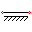
\includegraphics[width=0.4\linewidth]{tline}
\end{center}
\label{fig:TransLine}
\caption{ideal transmission line}
\end{figure}
\FloatBarrier

Applying $\textrm{I} + Z_L\cdot \textrm{II}$ and $\textrm{I} -
Z_L\cdot \textrm{II}$ to the above equation system and using the
following transformations
\begin{align}
\cosh{x} + \sinh{x} &= \dfrac{e^x + e^{-x}}{2} + \dfrac{e^x - e^{-x}}{2} = e^x\\
\cosh{x} - \sinh{x} &= \dfrac{e^x + e^{-x}}{2} - \dfrac{e^x - e^{-x}}{2} = e^{-x}
\end{align}

yields
\begin{align}
\label{eq:tl_v1}
V_1 &= V_2\cdot e^{-\gamma\cdot l} + Z_L\cdot \left(I_1 + I_2\cdot e^{-\gamma\cdot l}\right)\\
\label{eq:tl_v2}
V_2 &= V_1\cdot e^{-\gamma\cdot l} + Z_L\cdot \left(I_2 + I_1\cdot e^{-\gamma\cdot l}\right)
\end{align}

whereas $\gamma$ denotes the propagation constant $\alpha + j\beta$,
$l$ the length of the transmission line and $Z_L$ the line impedance.

\addvspace{12pt}

These equation can be transformed from the frequency domain into the
time domain using the inverse Fourier transformation.  The frequency
independent loss $\alpha \ne f\left(\omega\right)$ gives the constant
factor 
\begin{equation}
A = e^{-\alpha\cdot l}
\end{equation}

The only remaining frequency dependent term is
\begin{equation}
e^{-j\beta\cdot l} = e^{-j\omega\cdot\tau}
\;\;\;\; \textrm{with} \;\;\;\;
\beta = \dfrac{\omega}{v_{ph}} = \dfrac{\omega}{c_0} = \dfrac{\omega\cdot \tau}{l}
\end{equation}

which yields the following transformation
\begin{equation}
f\left(\omega\right)\cdot e^{-\gamma\cdot l} =
A\cdot f\left(\omega\right)\cdot e^{-j\omega\cdot\tau}
\Longleftrightarrow
A\cdot f\left(t - \tau\right)
\end{equation}

All the presented time-domain models with a frequency-independent
delay time are based on this simple transformation.  It can be applied
since the phase velocity $v_{ph} \ne f\left(\omega\right)$ is not a
function of the frequency.  This is true for all non-dispersive
transmission media (e.g. air or vacuum).  The given transformation can
now be applied to the eq. \eqref{eq:tl_v1} and eq. \eqref{eq:tl_v2}
defined in the frequency-domain to obtain equations in the
time-domain.

\addvspace{12pt}

The length $T_{end}$ of the memory needed by the ideal transmission
line can be easily computed by
\begin{equation}
T_{end} = \tau = \dfrac{l}{v_{ph}} = \dfrac{l}{c_0}
\end{equation}
whereas $c_0$ denotes the speed of light in free space (since there is
no dielectric involved during transmission) and $l$ the physical
length of the transmission line.

\addvspace{12pt}

The MNA matrix for a lossy (or lossless with $\alpha = 0$)
transmission line during the transient analysis is augmented by two
new rows and columns in order to consider the following branch
equations.
\begin{align}
V_1\left(t\right) = Z_L\cdot I_1\left(t\right) + A\cdot\left( Z_L\cdot I_2\left(t -\tau\right) + V_2\left(t -\tau\right)\right)\\
V_2\left(t\right) = Z_L\cdot I_2\left(t\right) + A\cdot\left( Z_L\cdot I_1\left(t -\tau\right) + V_1\left(t -\tau\right)\right)
\end{align}

Thus the MNA matrix entries can be written as
\begin{equation}
\begin{bmatrix}
0 & 0 & 1 & 0\\
0 & 0 & 0 & 1\\
1 & 0 & -Z_L & 0\\
0 & 1 & 0 & -Z_L
\end{bmatrix}
\cdot
\begin{bmatrix}
V_1\left(t\right)\\
V_2\left(t\right)\\
J_1\left(t\right)\\
J_2\left(t\right)
\end{bmatrix}
=
\begin{bmatrix}
I_1\left(t\right)\\
I_2\left(t\right)\\
A\cdot\left(V_2\left(t -\tau\right) + Z_L\cdot J_2\left(t -\tau\right)\right)\\
A\cdot\left(V_1\left(t -\tau\right) + Z_L\cdot J_1\left(t -\tau\right)\right)\\
\end{bmatrix}
\end{equation}

with $A$ denoting the loss factor derived from the constant (and
frequency independent) line attenuation $\alpha$ and the transmission
line length $l$.
\begin{equation}
A = e^{-\tfrac{\alpha}{2}\cdot l}
\end{equation}

\subsection{Components with frequency-dependent delay times and losses}
%\addcontentsline{toc}{subsection}{Components with frequency-dependent delay times and losses}

\section{Convergence}
%\addcontentsline{toc}{section}{Convergence}

Similar to the DC analysis convergence problems occur during the
transient analysis (see section \ref{sec:convergenceDC} on page
\pageref{sec:convergenceDC}) as well.  In order to improve the overall
convergence behaviour it is possible to improve the models on the one
hand and/or to improve the algorithms on the other hand.

\addvspace{12pt}

The implications during Newton-Raphson iterations solving the linear
equation system
\begin{equation}
\left[A\left(x^k\right)\right] \cdot \left[x^{k+1}\right] = \left[z\left(x^k\right)\right]
\end{equation}

are continuous device model equations (with continuous derivatives as
well), floating nodes (make the Jacobian matrix $A$ singular) and the
initial guess $x^0$.  The convergence problems which in fact occur are
local minimums causing the matrix $A$ to be singular, nearly singular
matrices and overflow problems.

\begin{figure}[ht]
\begin{center}
\includegraphics[width=0.9\linewidth]{convprob1}
\end{center}
\label{fig:ConvProb1}
\end{figure}
\FloatBarrier

\begin{figure}[ht]
\begin{center}
\includegraphics[width=0.9\linewidth]{convprob2}
\end{center}
\label{fig:ConvProb2}
\end{figure}
\FloatBarrier

\subsection{Limiting schemes}
%\addcontentsline{toc}{subsection}{Limiting schemes}

The modified (damped) Newton-Raphson schemes are based on the
limitation of the solution vector $x^k$ in each iteration.
\begin{equation}
x^{k+1} = x^k + \alpha\cdot \Delta x^{k+1}
\;\;\;\; \textrm{ with } \;\;\;\;
\Delta x^{k+1} = x^{k+1} - x^k
\end{equation}

One possibility to choose a value for $\alpha \in [0,1]$ is
\begin{equation}
\alpha = \dfrac{\gamma}{\left\lVert\Delta x^{k+1}\right\rVert_{\infty}}
\end{equation}

This is a heuristic and does not ensure global convergence, but it can
help solving some of the discussed problems.  Another possibility is
to pick a value $\alpha^k$ which minimizes the $L_2$ norm of the right
hand side vector.  This method performs a one-dimensional (line)
search into Newton direction and guarantees global convergence.
\begin{equation}
x^{k+1} = x^k + \alpha^k \cdot \Delta x^{k+1}
\;\;\;\; \textrm{ with an } \alpha^k \textrm{ which minimizes } \;\;\;\;
\left\lVert z\left(x^k + \alpha^k \cdot \Delta x^{k+1}\right)\right\rVert_2
\end{equation}

The one remaining problem about that line search method for
convergence improvement is its iteration into local minimums where the
Jacobian matrix is singular.  The damped Newton-Raphson method
``pushes'' the matrix into singularity as depicted in
fig. \ref{fig:ConvProb3}.
\begin{figure}[ht]
\centering
\includegraphics[width=0.55\linewidth]{convprob3}
\caption{singular Jacobian problem}
\label{fig:ConvProb3}
\end{figure}
\FloatBarrier

\subsection{Continuation schemes}
%\addcontentsline{toc}{subsection}{Continuation schemes}
\label{sec:continuation}

The basic idea behind this Newton-Raphson modification is to generate
a sequence of problems such that a problem is a good initial guess for
the following one, because Newton basically converges given a close
initial guess.

\addvspace{12pt}

The template algorithm for this modification is to solve the equation
system
\begin{align}
\left[A\right] \cdot \left[x\right] - \left[z\right] &= 0\\
F\left(x\left(\lambda\right), \lambda\right) &= 0
\end{align}

with the parameter $\lambda \in [0,1]$ given that
$x\left(\lambda\right)$ is sufficiently smooth.
$F\left(x\left(0\right), 0\right)$ starts the continuation and
$F\left(x\left(1\right), 1\right)$ ends the continuation.  The
algorithm outline is as follows: First solve the problem
$F\left(x\left(0\right), 0\right)$, e.g. set $\lambda = \Delta\lambda
= 0.01$ and try to solve $F\left(x\left(\lambda\right),
\lambda\right)$.  If Newton-Raphson converged then increase $\lambda$
by $\Delta\lambda$ and double $\Delta\lambda = 2\cdot \Delta\lambda$,
otherwise half $\Delta\lambda = 0.5\cdot \Delta\lambda$ and set
$\lambda = \lambda_{prev} + \Delta\lambda$.  Repeat this until
$\lambda = 1$.

\subsubsection{Source stepping}
%\addcontentsline{toc}{subsubsection}{Source stepping}

Applied to the solution of (non-linear) electrical networks one may
think of $\alpha \in [0,1]$ as a multiplier for the source vector $S$
yielding $S\left(\alpha\right) = \alpha S$.  Varying $\alpha$ form 0
to 1 and solve at each $\alpha$.  The actual circuit solution is done
when $\alpha = 1$.  This method is called source stepping.  The
solution vector $x\left(\alpha\right)$ is continuous in $\alpha$
(hence the name continuation scheme).

\subsubsection{Minimal derivative $\mathrm{g_{min}}$ stepping}
%\addcontentsline{toc}{subsubsection}{Minimal derivative $\mathrm{g_{min}}$ stepping}

Another possibility to improve convergence of almostly singular
electrical networks is the so called $g_{min}$ stepping, i.e. adding a
tiny conductance to ground at each node of the Jacobian $A$ matrix.
The continuation starts e.g. with $g_{min} = 0.01$ and ends with
$g_{min} = 0$ reached by the algorithm described in section
\ref{sec:continuation}.  The equation system is slightly modified by
adding the current $g_{min}$ to each diagonal element of the matrix
$A$.
